\chapter{Software implementation}\label{chap:imp}

\section{Design objectives}\label{sec:des_obj}
%St 1
%broad objectives
Our primary aim is to test and research mm-VLBI calibration, imaging and parameter estimation algorithms/strategies through the construction of a synthetic data simulation framework. To address the many questions within the wide scope of this objective, one must be able to setup and run a diverse set of experiments within the simulation framework. This places definite constraints on the software architechure. In particular, the framework should :


%specific objectives
\begin{itemize}
%framework for consistent implementation of the necessary signal corruptions  
 \item enable the implementation of the dominant classes of signal corruption within a formalism which ensures consistency with the causal signal transmission chain,
 %grmhd input
 \item be compatible with time-variable GRMHD source models which are to be used as inputs,
 %modularise - extendable
 \item be organised in a modular structure so that it is flexible, extendable and could be incorporated into other interferometric algorithms or vice-versa (e.g. a calibration or a parameter estimation algorithm),
  %modularise - diverse experiments
 \item the modular structure should also enable the construction and execution of arbitrary observations.
\end{itemize}

\section{Architechure and Workflow}\label{sec:arch}
%Intro and plan, How to meet objectives %st 1
In this section, we will review how the architechural design and workflow of the simulator has been designed to meet the above objectives. To fulfill the first objective, we cast signal corruptions in the RIME formalism (see section~\ref{sec:RIME}). This is not currently possible for the case of ISM-scattering, however we do apply it in the casually correct position in the signal transmission chain, with proper consideration given to non-communitivity of elements. The implementation of each signal corruption is described in the following subsections. The remaining objectives fall into the realm of software design and will be discussed in this subsection. 


%Language
We have chosen to write the high level simulation code using the \textsc{Python} language. \textsc{Python} is a general purpose language, is geared towards readability, and is well supported by a comprehensive library and wide user base, particularly within astronomy. Even though the higher level functionality is written in \textsc{Python}, the bulk of the computational load is called through subroutines which are written in the more computationally efficient {\sc C++} language.


%Meqtrees-description
We use the interferometric toolbox, {\sc MeqTrees} \citep{Noordam_2010}, which can simulate and calibrate radio interferometic data through evaluation of a user-defined RIME. The evaluation draws on directed-acyclic-graphs (or compute trees) where each element of the graph can process a multi-dimensional grid of values (typically specified along axes of $\nu$ and $t$).
%our usuage of it
Although we have decided to construct a large portion of our RIME outside of {\sc MeqTrees}, we call prebuilt {\sc MeqTrees} RIMEs to augment our pipeline in two ways. Firstly to perform the Fourier transform  to generate visibilities from the input sky model (FFT for fits files; DFT for parametric sources), where degridding and interpolation steps are also called when the FFT is used. The second is to simulate the primary beam and antenna pointing error, which will be discussed later in this chapter. On a side note, use of \textsc{MeqTrees} and \textsc{measurement set} also lends itself to investigating a range of different techniques that are used in other areas of interferometry \citep*[e.g.][]{Smirnov_2015}.


%data format choice
Our data formats of choice are: {\sc fits} for image cubes and the {\sc measurement set}\footnote{https://casa.nrao.edu/Memos/229.html} ({\sc ms}) for visibilities. We use {\sc ms} as our data format as it is directly accessible in {\sc Python} via the {\sc pyrap} library and is the data format used by {\sc MeqTrees}. Although in the mm-VLBI subfield, other data formats are currently still more popular than the {\sc ms}, i.e. {\sc fitsidi}, {\sc uvfits} or {\sc iofits}, largely due to the lack of a fringe-fitter in {\sc casa} and incomplete meta-data fields. However,  thanks to development at the Joint Institute for VLBI in Europe (JIVE), we expect this to change in {\sc casa v5}. 


%Highest level architechure : Distinction between framework and driver and how they link %st 1
To create a flexible and modular structure necessary to be able to run a diversity of experiments, the software implementation is divided into 2 components:
\begin{itemize}
 \item an object-oriented framework into which is programmed the logic of each individual step in the signal propagation chain,
 \item a driver script which initialises the most abstract class in the framework with the required inputs and determines the signal propagation chain relevant to that particular pipeline.
\end{itemize}
The conceptual flow diagram of one realisation of a {\sc meqsilhouette} simulation pipeline is shown in Fig.~\ref{flow}. To emphasise, the framework is not restricted to this sequence of operations, allowing the exact pipeline to be quite general. Note that this diagram is not entirely accurate as antenna pointing errors are not compatible with the {\sc fits} sky model output by the ISM scattering module.


%Inputs %st 1
All inputs to the simulator are specified by a configuration file (.json text file), containing a dictionary (see table~\ref{tab:parameters} as an example), which is the sole input to the driver script. This dictionary contains everything needed by the pipeline to determine the particular observation configuration (frequency, bandwidth, start time, etc), which signal corruption implementation should be employed and where the sky model, station weather information and antenna table are located in the filesystem. The antenna table is in the {\sc ms} format, and can readily be created or altered using the {\sc pyrap} library using the station coordinates. The primary sky model used is a time-ordered list of {\sc fits} images, where each image represents the source total intensity over a time interval $\Delta t_{\rm src} = t_{\rm obs}/N_{\rm src}$, where $t_{\rm obs}$ is the observation length and $N_{\rm src}$ is the number of source images \citep{Blecher_2016}. Currently the pipeline only supports total intensity and the conversion of the pipeline to support full Stokes is discussed in section~\ref{sec:improv}. A variation of the pipeline has also been written which uses a parametric source model consisting of Gaussians or point sources as the sky model. This functionality was needed for the simulation of pointing errors as the {\sc MeqTrees} beams model does not support the {\sc fits} sky model.

\begin{figure*}[h!]
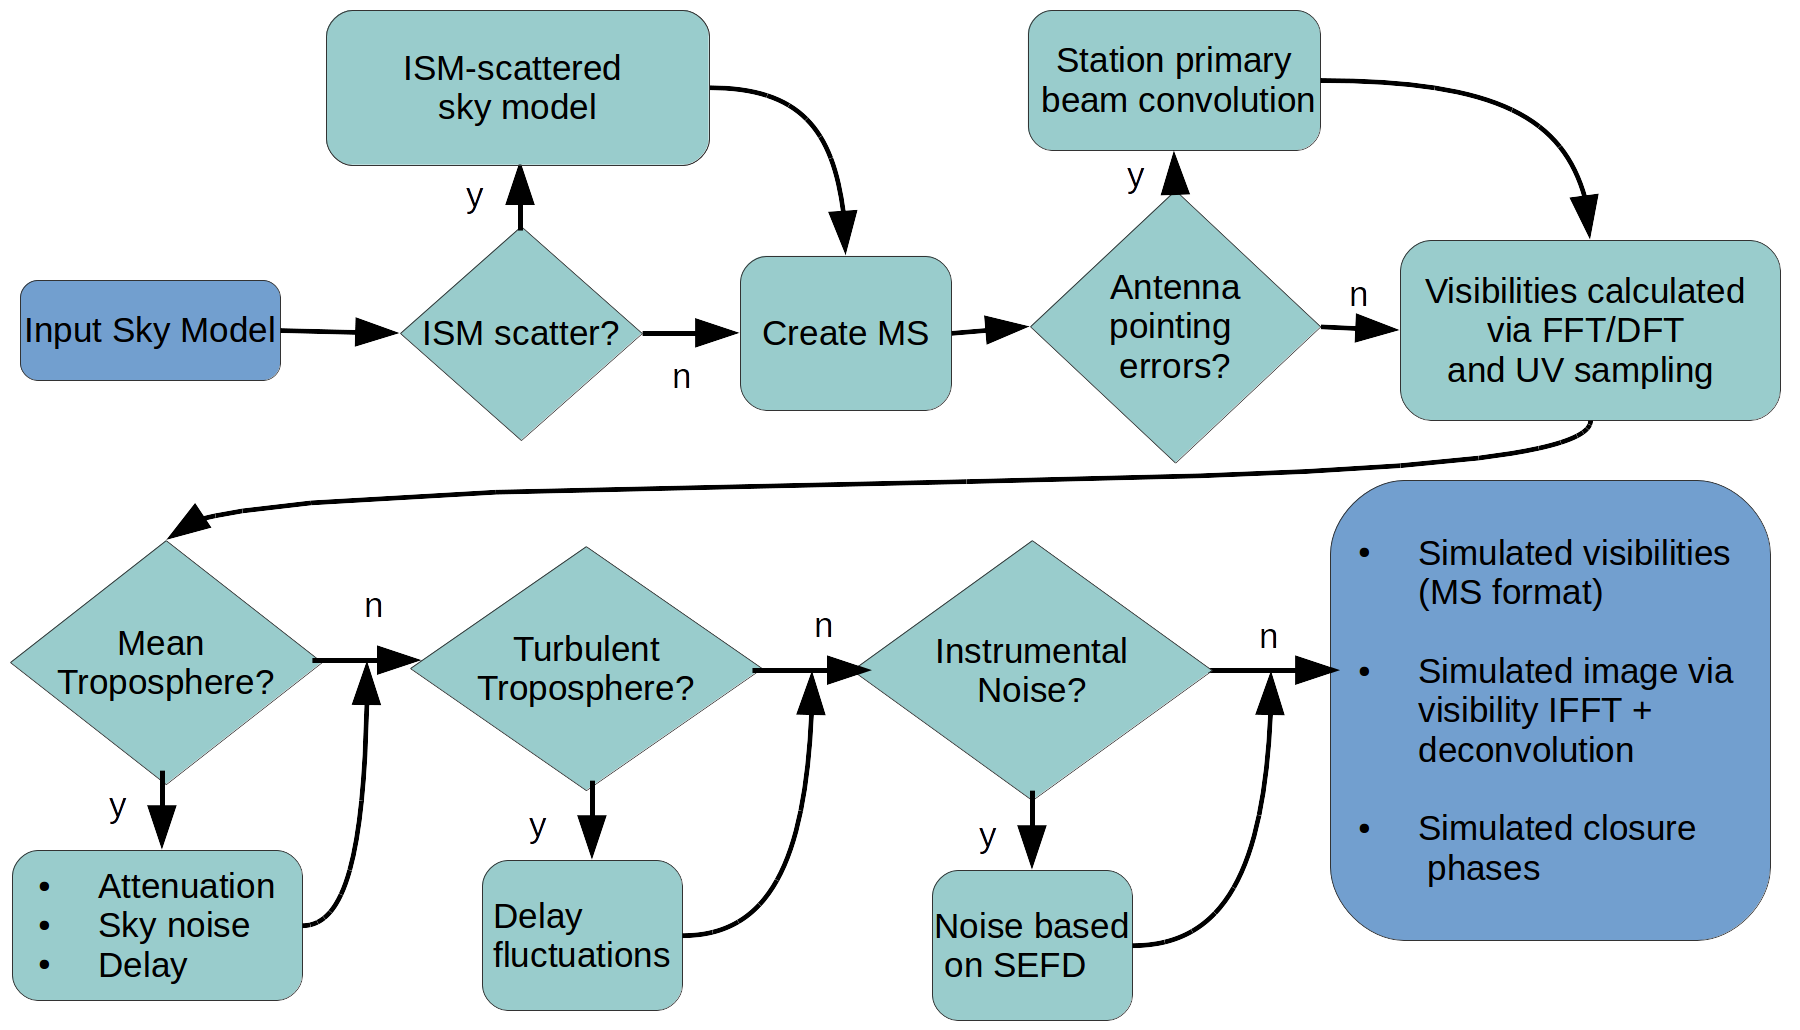
\includegraphics[width=\columnwidth]{Images/flow_full2}
\caption{Flow diagram showing basic sequence of a \textsc{meqsilhouette} simulation pipeline. The specific sequence is determined by the driver script whereas the logic of each step is contained in an object-oriented framework. The details of the station information, observation strategy, tropospheric and ISM conditions are specified in a user-defined input configuration file. The pipeline is extendable, allowing any additional, arbitrary Jones matrices to be incorporated. \label{flow}%
}
\end{figure*}


\begin{table}
\caption{{\bf Top section:} keywords of the input configuration dictionary used in a standard simulation similar to that depicted in Fig.~\ref{flow} but without antenna pointing errors. The variable names have been expanded for clarity and keywords which have boolean values have written as questions. In practice, most of these keywords are predeced by an index, which allows this dictionary to be filter into several subdictionaries which can be easily passed to functions or classes. {\bf Bottom section:} the headings of station weather table whose path is indicated in the input dictionary.}
\label{tab:parameters}
\begin{tabular}{ll}
\hline
parameter&comment\\
\hline
input fits folder path&folder containing intrinsic sky models in {\sc fits} format\\
antenna table path&antenna table in {\sc casa} format\\
integration time (seconds)&time averaging interval for each visibility data point\\
start time&time system (e.g. UTC) and the observation start date and time\\
channel width (GHz)&\\
number of channels& currently {\sc meqsilhouette} can only simulate 1 spectral window\\
number of scans & split observation for into different scans of equal length\\
scan lag (hours)& lag time between scans\\
elevation limit (radians) & limit below which all data is automatically flagged\\
central observing frequency (GHz)& \\
total observation length (hours)&\\
apply ISM scattering?&\\
number of ISM screen realisations&\\
ISM screen speed&will come into effect only for multiple ISM screens\\
ISM ${\rm N_{pix}}$& size of screen\\
apply atmospheric attentuation?&\\
add thermal noise?&calculated with station SEFD\\
apply atmospheric thermal noise?& derived from atmospheric brightness temperature \\
apply tropospheric turbulence-induced phase noise?&applies to all antennae\\
apply mean atmospheric time delays?&percentage tropospheric phase \\
output image pixel size&output image ${\rm N_{pix}}$\\
station information file path& station dependent details, headings of this table shown below
\hline
\hline
station&coherence time\\
sefd&pvw\\
ground pressure&ground temperature\\
\end{tabular} 
\end{table}

%Outputs and Data products %st 1
The primary outputs of the pipeline are an interferometric dataset in MS format along with the closure phases and uncertainties, a dirty and/or deconvolved image, and tropospheric phase delays, opacities etc. Closure phases and uncertainties are calculated in a model-dependent way as described by section~\ref{data_products}. The modular structure of the pipeline allows for additional imaging and deconvolution algorithms to be easily appended to the final data processing steps. Noting that there are other data formats widely used in mm-VLBI, we make use of the {\sc casa} task for conversion to {\sc uvfits}. Similiarly other data products can be easily produced as needed e.g. polarisation ratios.


%Overview of the workflow

%workflow fig : example of a pipeline %st 1

\begin{figure*}
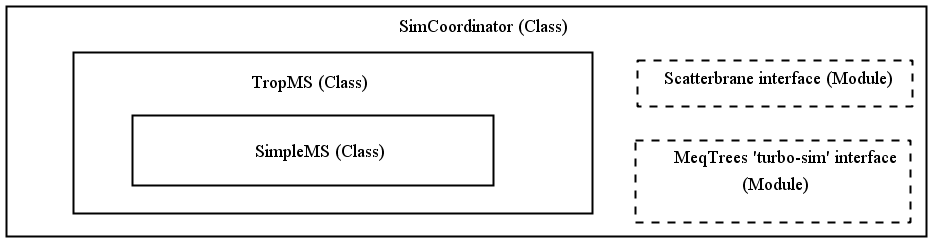
\includegraphics[width=\columnwidth]{Images/Class_module_structure}
\caption{The basic class and module structure of the {\sc meqsilhouette} implementation. Solid lines represent a class while dashed lines represent a module. The \emph{SimCoordinator} class is initialised in the driver script. \label{class_struc}%
}
\end{figure*}

%Framework - details %st 1
%ms creation 
An important step to reproduce realistic observations is to be able create a comprehensive MS with arbitrary scan lengths, start times, channel and bandwidth structure. This is performed using the {\sc simms}\footnote{https://github.com/radio-astro/simms} tool. {\sc simms} provides an easy to use command line interface to construct a general MS, given the appropriate antenna table. The call to {\sc simms} is located within the driver script. 

%%Class diagram
% Calculation and & back end & object orientation
%SimpleMS
In order to make the framework as clean and  modular as possible we have made extensive use of object orientation, see Fig.~\ref{class_struc} for a basic overview. The first major class, \emph{SimpleMS}, was intended to abstract and modularise the MS and MS-only derived attributes (e.g. visibility data and station positions) and methods (e.g. functions to calculate station elevations and closure phases) as well as expose these attributes and methods more efficiently than following {\sc pyrap} procedures which become verbose when used frequently. This is especially useful when accessing baseline-indexed quantities. 

%TropMS
The second MS-related class, \emph{TropMS}, handles the calculations relevant to tropospheric and thermal noise corruptions. This class is a child of {\it SimpleMS} and is initialised with weather and station information. Note that a child contains all the methods and attributes of its parent. This allows the tropospheric corruption implementation to use, whilst being separated from, the core MS functionality. The details of the tropospheric corruption are provided in section~\ref{sec:trop_imp}. 

%SimCoordinator
The third MS-related class, \emph{SimCoordinator}, is a child of the {\it TropMS} class. {\it SimCoordinator} is designed to make a simulation, with an arbitrary experimental setup, easy and efficient to construct and execute on a high level. It is the only MS class directly initialised in the driver script and hence the low level functionality and attributes of its parents are abstracted from the user. In addition to inherited functionality, {\it SimCoordinator} can call the ISM-scattering task (see subsection~\ref{sec:ism_imp}), and {\sc MeqTrees} simulation functionality.
 

\subsection{ISM scattering}\label{sec:ism_imp}
%Pr 1 St 1

%Link back to theory %st 1
As described in section~\ref{sec:ism_scat}, observations of Sgr~A$^\star$ at sub(mm) wavelengths is subject to ISM scattering in the strong scattering regime. Due to the size of Sgr~A* at mm-wavelengths, a single epoch observation of the scattering screen is further defined as falling into the \emph{average regime}, wherein diffractive scintillation is averaged out but refractive scintillation is still present. As mm-VLBI observations can resolve the scatter-broadened image of Sgr~A$^\star$, an implementation of scattering is needed which approximates the subtle changes in its extended source structure. Such an approximation has been implemented in the \textsc{Python}-based \textsc{Scatterbrane}\footnote{http://krosenfeld.github.io/scatterbrane} package, and is based on \citet*{Johnson_2015a}. In this algorithm a phase screen is created based on the two dimensional spatial power spectrum  \citep*[see][Appendix C]{Johnson_2015a} which incorporates inner and outer turbulent lengths scales. With the screen generated, the original image is scattered according to equation~\ref{eq:scatterbrane}. In practice equation~\ref{eq:scatterbrane} is implemented using an interpolation function which is modified by the values on the phase screen. {\sc ScatterBrane} allows variation in all parameters (see table~\ref{tab:parm_ism}) associated with the scattering screen which is essential as aspects of the scattering towards the Galactic Centre are still unconstrained \citep[e.g.][]{Gwinn_2014}.

%scatterbrane inputs and generality %st 1
\begin{table}
\centering
\caption{The list of the parameters, aside from the source model, needed to initialise and run {\sc ScatterBrane}. Time variability is made possible as $N_{\rm pix}$ can be a 2-tuple (i.e. a rectangular screen can be created).
}
\begin{tabular}{ll}\label{tab:parm_ism}
$r_0$            & $N_{\rm pix}$ \\
$r_{\rm in}$     & principal angle             \\
$r_{\rm out}$    & anisotropy of scattering kernel    \\
$D_{\rm os}$     & $\lambda$        \\
$R$              & $\beta$          \\
screen resolution &               
\end{tabular}
\end{table}



%Integration of Scatterbrane %st 1
We include the {\sc ScatterBrane} software, which has already yielded important context for mm-VLBI observations towards Sgr~A$^\star$ \citep[e.g.][]{Ortiz_2016}, within the {\sc meqsilhouette} framework. Our ISM module interfaces the \textsc{Scatterbrane} code within an interferometric simulation pipeline. This module enables simultaneous use of time-variable ISM scattering and time-variable intrinsic source structure within a single framework. The user is able to select a range of options relating to the time-resolution and epoch interpolation/averaging of both. By default, if the time resolution chosen to sample the source variability $\Delta t_{\rm src}$ and screen variability $\Delta t_{\rm ism}$ are unequal, we set  
\begin{itemize}
 \setlength\itemsep{1em}
\item $\Delta t_{\rm ism}=\Delta t_{\rm src}$ \qquad \qquad if \qquad  $\Delta t_{\rm src} < \Delta t_{\rm ism}$
\item $\Delta t_{\rm ism}={\rm R}(\frac{\Delta t_{\rm src}}{\Delta t_{\rm ism}})\Delta t_{\rm src}$ \ if \qquad  $\Delta t_{\rm src} > \Delta t_{\rm ism}$,
\end{itemize}
where ${\rm R}$ rounds the fraction to the nearest integer.  This modification to the ISM sampling resolution avoids interpolation between different snapshots of the intrinsic source structure.


\subsection{Atmospheric corruption simulator}\label{sec:trop_imp}
%Pr 1 St 1

%average/turbulent split st 1
Our focus in this module is to model the three primary, interrelated (see section~\ref{sec:prop_fund}) observables which are the most relevant to mm-VLBI: turbulence-driven fluctuations in the visibility phase $\delta \phi$; signal attenuation due to the atmospheric opacity $\tau$; and the increase in system temperature due to atmospheric emission at a brightness temperature $T_{\rm atm}$ due to non-zero opacity. Our approach is to model these observables as being separable into mean and turbulent components which are simulated independently \citep{Blecher_2016}. The mean tropospheric simulation module performs radiative transfer with a detailed model of the electromagnetic spectrum of each atmospheric constituent (i.e. ${\rm O_2}$, {\rm $H_2O$}, ${\rm N_2}$, etc.). The turbulent simulation module uses a scattering formalism to account for the decoherence that results from power-law turbulence.

%Implementation details of ATM st 1
%what it does and how it fits into the broader scheme
As described in section~\ref{sec:atm_theory}, we use the {\sc atm} package to perform radiative transfer through the realisation of the mean atmosphere. 
%inputs
In order to calculate atmospheric temperature and pressure profiles, {\sc atm} is input several station dependent parameters, namely, ground temperature and pressure, PWV depth, water vapour scale height, tropospheric lapse rate  and altitude. The lapse rate refers to the linear relation at which temperature decreases with height. Through experimentation, we have found that the first 3 variables most significantly effect the results of the simulation and opt to keep the latter variables at their default values which were set for application to ALMA. 
%outputs
The outputs of this procedure are mean values for opacity, time delay and atmospheric brightness temperature at each station towards zenith. Both opacity and time delay are separated into wet (water vapour) and dry (other) components. Furthermore, The time delay is subdivided into dispersive and non-dispersive  components. These outputs are calculated for a list of frequency values. Hence, the non-dispersive component of the mean atmosphere is accounted for.
%interface details
We perform this calculation using representative climate conditions taken from the literature. This final step is to account for elevation effects by multiplying by the airmass $1/\sin\theta$. Since all stations have elevation limits of $>10^\circ$, this is a reasonable assumption.

%phase turbulence st 1
%what it does and How it fits into the broader scheme
Following from section~\ref{sec:turb_theory}, we derive a weak scattering formalism to calculate station dependent visibility phase variations which result from observing through a turbulent troposphere. Specifically, we simulate random walks in visibility phase with variance given by equation~\ref{eq:turb_final} for each antenna. These phase-time series are combined to form a multiplicative complex gain corruption, with amplitude of unity i.e. a diagonal Jones matrix. In section~\ref{sec:can_sim} we explore the effect of the mean and turbulent atmosphere on observables.


This framework would enable the exploration of an arbitrary or typical range of weather conditions on mm-VLBI observations for each unique station.

\subsection{Antenna pointing error simulator}\label{sec:point_imp}
%St1

%The pointing implementation in MeqTrees, WSRT beams, approximating the LMT error
To simulate pointing errors, we use the implementation built into the {\sc MeqTrees} package. This functionality includes the capability to convolve station primary beams with the sky model, which is implemented as an E-Jones matrix in the RIME (see section~\ref{sec:instrument}). The beam models available through this function are sinc, Gaussian and the analytic WSRT beam model. The standard beam model which we will make use of is the analytic WSRT beam model \citep{Popping_2008} 
\begin{equation}\label{eq:wsrt_beam}
E(l, m) = \cos^3(C\nu \rho),\qquad   \rho \equiv \sqrt{\delta l_p^2 + \delta m_p^2},
\end{equation}
where $C$ is a constant, with value $C \approx 65$~GHz$^{-1}$ for a dish diameter of 25~m. Note that the power beam $EE^H$ becomes $\cos^6(\rho)$.  One drawback of the {\sc MeqTrees} implementation is that it is incompatible with the {\sc fits} format and so we are at present limited to point and Gaussian parameteric sources for the pointing error simulations. However this is not a significant issue as the primary beam should be constant across the synthesised FOV, effectively reducing to a Direction Independent Effect (DIE), and hence source structure is unimportant to pointing error analysis within the mm-VLBI framework.


%pointing models
Furthermore, {\sc Meqtrees} allows a constant offset or time-variable primary beam, where the time variability can be either a polynomial (up to third order) or a sinusoid. We have opted to use only the sinusoidal variability for simplicity. To simulate stochastic variability i.e. pointing error due to slew between calibrator and source, we use a constant offset which is resampled per user-specified time interval. In section~\ref{sec:can_sim} we demonstrate the effect of constant, sinusoidal and stochastic pointing error variablility on the Large Millimeter Telescope (LMT) within the context of the EHT array.

